\documentclass{beamer}
\usepackage[utf8]{inputenc}
\usepackage{graphicx, epsfig}
\usepackage{amsmath,mathrsfs,amsfonts,amssymb}
%\usepackage{subfig}
\usepackage{floatflt}
\usepackage{epic,ecltree}
\usepackage{mathtext}
\usepackage{fancybox}
\usepackage{fancyhdr}
\usepackage{multirow}
\usepackage{enumerate}
\usepackage{epstopdf}
\usepackage{multicol}
\usepackage{algorithm}
\usepackage[noend]{algorithmic}
\def\algorithmicrequire{\textbf{Input:}}
\def\algorithmicensure{\textbf{Output:}}
\usetheme{default}%{Singapore}%{Warsaw}%{Warsaw}%{Darmstadt}
\usecolortheme{default}
\setbeamerfont{title}{size=\Huge}
\setbeamertemplate{footline}[page number]{}
\setbeamerfont{title}{size=\Huge}
\beamertemplatenavigationsymbolsempty

% latin bold lower
\newcommand{\ba}{\mathbf{a}} 
\newcommand{\bc}{\mathbf{c}} 
\newcommand{\be}{\mathbf{e}} 
\newcommand{\bh}{\mathbf{h}} 
\newcommand{\bp}{\mathbf{p}} 
\newcommand{\bt}{\mathbf{t}} 
\newcommand{\bu}{\mathbf{u}} 
\newcommand{\bv}{\mathbf{v}} 
\newcommand{\bw}{\mathbf{w}} 
\newcommand{\bx}{\mathbf{x}} 
\newcommand{\by}{\mathbf{y}} 
\newcommand{\bz}{\mathbf{z}} 

% latin bold upper
\newcommand{\bA}{\mathbf{A}} 
\newcommand{\bC}{\mathbf{C}} 
\newcommand{\bI}{\mathbf{I}} 
\newcommand{\bM}{\mathbf{M}} 
\newcommand{\bT}{\mathbf{T}} 
\newcommand{\bU}{\mathbf{U}} 
\newcommand{\bW}{\mathbf{W}} 
\newcommand{\bX}{\mathbf{X}} 
\newcommand{\bY}{\mathbf{Y}} 
\newcommand{\bZ}{\mathbf{Z}} 

% latin cal upper
\newcommand{\cL}{\mathcal{L}} 
\newcommand{\cN}{\mathcal{N}} 
\newcommand{\cS}{\mathcal{S}} 
\newcommand{\cT}{\mathcal{T}} 
\newcommand{\cW}{\mathcal{W}} 
\newcommand{\cX}{\mathcal{X}} 
\newcommand{\cZ}{\mathcal{Z}} 

% latin cal upper
\newcommand{\bbE}{\mathbb{E}} 
\newcommand{\bbP}{\mathbb{P}} 
\newcommand{\bbR}{\mathbb{R}} 

% greek bold lower
\newcommand{\bepsilon}{\boldsymbol{\epsilon}} 
\newcommand{\btheta}{\boldsymbol{\theta}} 
\newcommand{\blambda}{\boldsymbol{\lambda}} 
\newcommand{\bmu}{\boldsymbol{\mu}} 
\newcommand{\bsigma}{\boldsymbol{\sigma}} 
\newcommand{\bphi}{\boldsymbol{\phi}} 

% greek bold upper
\newcommand{\bSigma}{\boldsymbol{\Sigma}} 

\DeclareMathOperator*{\argmin}{arg\,min}
\DeclareMathOperator*{\argmax}{arg\,max}

\newcommand{\createdgmtitle}[1]{\title[\hbox to 56mm{Deep Generative Models  \hfill\insertframenumber\,/\,\inserttotalframenumber}]
	{\vspace{1cm} \\ Deep Generative Models \\ Lecture #1 \\ \vspace{-0.5cm}}
	\author{Roman Isachenko \\ \vspace{-0.5cm}}
	\institute{
\includegraphics[width=3cm]{../utils/ozonmasterslogo}
	\\Ozon Masters
	}
	\date{Spring, 2021}
}

\newcommand\myfootnote[1]{%
  \tikz[remember picture,overlay]
  \draw (current page.south west) +(1in + \oddsidemargin,0.5em)
  node[anchor=south west,inner sep=0pt]{\parbox{\textwidth}{%
      \rlap{\rule{10em}{0.4pt}}\raggedright\scriptsize#1}};}

\newcommand\myfootnotewithlink[2]{%
  \tikz[remember picture,overlay]
  \draw (current page.south west) +(1in + \oddsidemargin,0.5em)
  node[anchor=south west,inner sep=0pt]{\parbox{\textwidth}{%
      \rlap{\rule{10em}{0.4pt}}\raggedright\scriptsize\href{#1}{\textit{#2}}}};}
\createdgmtitle{2}
%--------------------------------------------------------------------------------
\begin{document}
%--------------------------------------------------------------------------------
\begin{frame}
%\thispagestyle{empty}
\titlepage
\end{frame}
%=======
\begin{frame}{Recap of previous lecture}
	We are given i.i.d. samples $\{\bx_i\}_{i=1}^n \in X$ (e.g. $X = \bbR^m$) from unknown distribution $\pi(\bx)$.
	\begin{block}{Goal}
		We would like to learn a distribution $\pi(\bx)$ for 
		\begin{itemize}
			\item evaluating $\pi(\bx)$ for new samples (how likely to get object $\bx$?);
			\item sampling from $\pi(\bx)$ (to get new objects $\bx \sim \pi(\bx)$).
		\end{itemize}
	\end{block}
	\begin{block}{Challenge}
		Data is complex and high-dimensional.
	\end{block}
	\begin{block}{MLE problem}
	Fix probabilistic model $p(\bx | \btheta)$~-- a set of parameterized distributions, such that $p(\bx | \btheta) \approx \pi(\bx)$.
	
		\vspace{-0.3cm}
		\[
		\btheta^* = \argmax_{\btheta} p(\bX | \btheta) = \argmax_{\btheta} \prod_{i=1}^n p(\bx_i | \btheta) = \argmax_{\btheta} \sum_{i=1}^n \log p(\bx_i | \btheta).
		\]
		\vspace{-0.1cm}
	\end{block}
\end{frame}
\begin{frame}{Recap of previous lecture}
	\begin{block}{Likelihood as product of conditionals}
		Let $\bx = (x_1, \dots, x_m)$, $\bx_{1:i} = (x_1, \dots, x_i)$. Then 
		\[
		p(\bx | \btheta) = \prod_{i=1}^m p(x_i | \bx_{1:i - 1}, \btheta); \quad 
		\log p(\bx | \btheta) = \sum_{i=1}^m \log p(x_i | \bx_{1:i - 1}, \btheta).
		\]
	\end{block}
	\vspace{-0.3cm}
	\begin{block}{MLE problem for autoregressive model}
		\vspace{-0.5cm}
		\[
		\btheta^* = \argmax_{\btheta} p(\bX | \btheta) = \argmax_{\btheta} \sum_{i=1}^n \sum_{j=1}^m \log p(x_{ij} | \bx_{i, 1:j - 1}\btheta).
		\]
		\vspace{-0.5cm}
	\end{block}
	\begin{block}{Sampling}
		\vspace{-0.5cm}
		\[
			\hat{x}_1 \sim p(x_1 | \btheta), \quad \hat{x}_2 \sim p(x_2 | \hat{x}_1, \btheta), \dots, \quad \hat{x}_m \sim p(x_m | \hat{\bx}_{1:m-1}, \btheta)
		\]
		New generated object is $\hat{\bx} = (\hat{x}_1, \hat{x}_2, \dots, \hat{x}_m)$.
	\end{block}
\end{frame}
%=======
\begin{frame}{Generative models zoo}
    \begin{figure}
        \centering
        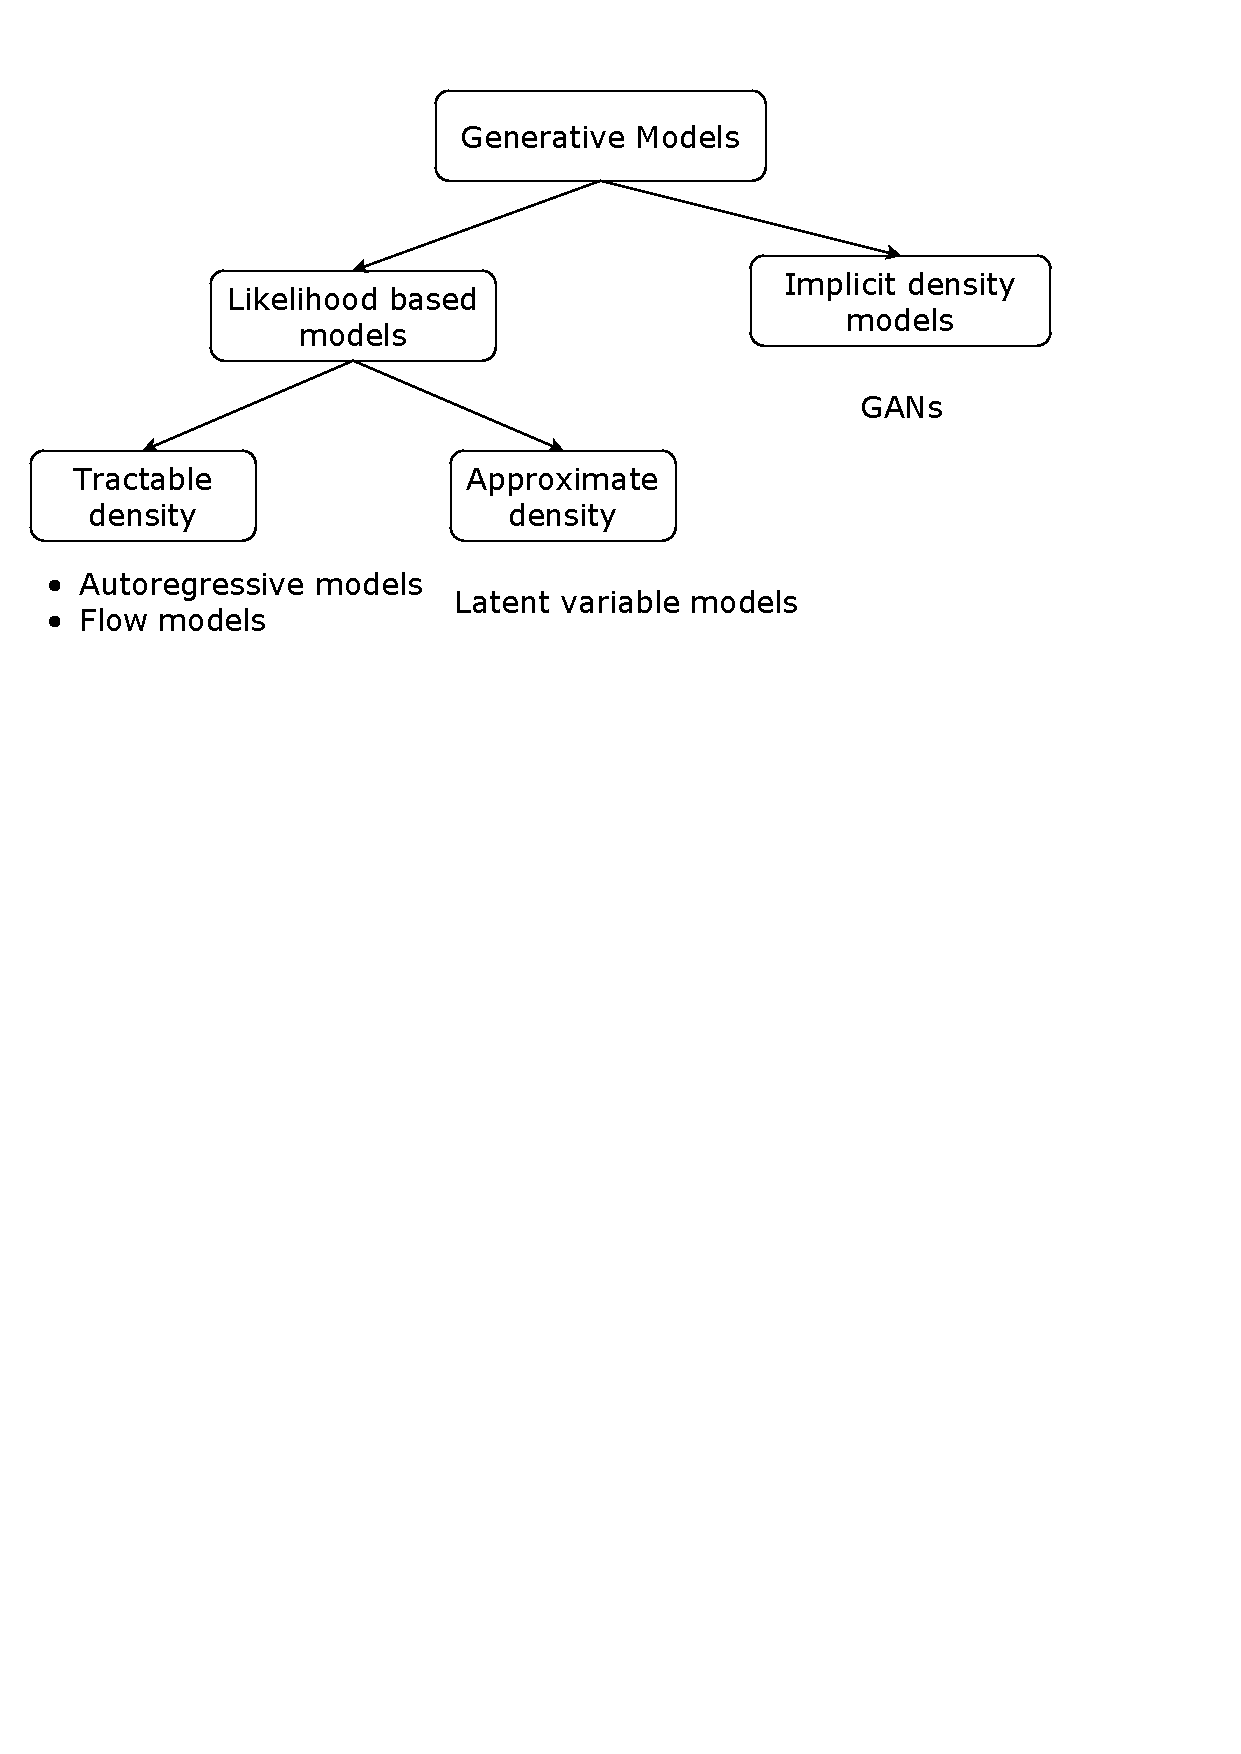
\includegraphics[width=1.0\linewidth]{figs/generative_models_zoo.pdf}
        \label{fig:generative_models_zoo}
    \end{figure}
\end{frame}
%=======
\begin{frame}{Bayesian framework}
	\begin{block}{Bayes theorem}
		\[
			p(\bt | \bx) = \frac{p(\bx | \bt) p(\bt)}{p(\bx)} = \frac{p(\bx | \bt) p(\bt)}{\int p(\bx | \bt) p(\bt) d \bt} 
		\]
		\begin{itemize}
			\item $\bx$ -- observed variables, $\bt$ -- unobserved variables (latent variables/parameters);
			\item $p(\bx | \bt)$ -- likelihood;
			\item $p(\bx) = \int p(\bx | \bt) p(\bt) d \bt$ -- evidence;
			\item $p(\bt)$ -- prior distribution, $p(\bt | \bx)$ -- posterior distribution.
		\end{itemize}
	\end{block}
	\begin{block}{Meaning}
		We have unobserved variables $\bt$ and some prior knowledge about them $p(\bt)$. Then, the data $\bx$ has been observed. 
		Posterior distribution $p(\bt | \bx)$ summarizes the knoweldge after the obbservations.
	\end{block}
\end{frame}
%=======
\begin{frame}{Bayesian framework}
	Let consider the case, where the unobserved variables $\bt$ is our model parameters $\btheta$.
	\begin{itemize}
		\item $\bX = \{\bx_i\}_{i=1}^n$ -- observed samples;
		\item $p(\btheta)$ -- prior parameters distribution (we treat model parameters $\btheta$ as random variables).
	\end{itemize}
	\begin{block}{Posterior distribution}
		\[
			p(\btheta | \bX) = \frac{p(\bX | \btheta) p(\btheta)}{p(\bX)} = \frac{p(\bX | \btheta) p(\btheta)}{\int p(\bX | \btheta) p(\btheta) d \btheta} 
		\]
		\vspace{-0.2cm}
	\end{block}
	\begin{block}{Bayesian inference}
		\vspace{-0.2cm}
		\[
			p(\bx | \bX) = \int p(\bx | \btheta) p(\btheta | \bX) d \btheta
		\]
	\end{block}
 	Note the difference from
	 	\[
	 		p(\bx) = \int p(\bx | \btheta) p(\btheta) d \btheta.
	 	\]
\end{frame}
%=======
\begin{frame}{Bayesian framework}
	\begin{block}{Posterior distribution}
		\[
		p(\btheta | \bX) = \frac{p(\bX | \btheta) p(\btheta)}{p(\bX)} = \frac{p(\bX | \btheta) p(\btheta)}{\int p(\bX | \btheta) p(\btheta) d \btheta} 
		\]
		\vspace{-0.2cm}
	\end{block}
	\begin{block}{Bayesian inference}
		\vspace{-0.2cm}
		\[
		p(\bx | \bX) = \int p(\bx | \btheta) p(\btheta | \bX) d \btheta
		\]
	\end{block}
	If evidence $p(\bX)$ is intractable (due to multidimensional integration), we can't get posterior distribution and perform the precise inference.
    \begin{block}{Maximum a posteriori (MAP) estimation}
    \vspace{-0.2cm}
    \[
        \btheta^* = \argmax_{\btheta} p(\btheta | \bX) = \argmax_{\btheta} \bigl(\log p(\bX | \btheta) + \log p(\btheta) \bigr)
    \]
    \end{block}
\end{frame}
%=======
\begin{frame}{Bayesian framework}
	\begin{block}{MAP estimation}
		\vspace{-0.2cm}
		\[
		\btheta^* = \argmax_{\btheta} p(\btheta | \bX) = \argmax_{\btheta} \bigl(\log p(\bX | \btheta) + \log p(\btheta) \bigr)
		\]
	\end{block}
	Estimated $\btheta^*$ is a deterministic variable, but we could treat it as a random variable with density $p(\btheta | \bX) = \delta(\btheta - \btheta^*)$.
	\begin{block}{Dirac delta function}
		\[
			\delta(x) = 
			\begin{cases}
				+\infty, \quad x = 0; \\
				0, \quad x \neq 0;
			\end{cases} \quad 
			\int f(x) \delta (x - y) dx = f(y).
		\]
	\end{block}
	\begin{block}{MAP inference}
		\[
			p(\bx | \bX) = \int p(\bx| \btheta) p(\btheta | \bX ) d \btheta \approx p(\bx | \btheta^*).
		\]
	\end{block}
\end{frame}
%=======
\begin{frame}{Latent variable models (LVM)}
    \begin{block}{MLE problem}
    \vspace{-0.5cm}
    \[
        \btheta^* = \argmax_{\btheta} p(\bX | \btheta) = \argmax_{\btheta} \prod_{i=1}^n p(\bx_i | \btheta) = \argmax_{\btheta} \sum_{i=1}^n \log p(\bx_i | \btheta).
    \]
    \vspace{-0.5cm}
    \end{block}
    \begin{block}{Challenge}
    $p(\bx | \btheta)$ could be intractable.
    \end{block}
    \begin{block}{Extend probabilistic model}
    Introduce latent variable $\bz$ for each sample $\bx$
    \[
        p(\bx, \bz | \btheta) = p(\bx | \bz, \btheta) p(\bz); \quad 
        \log p(\bx, \bz | \btheta) = \log p(\bx | \bz, \btheta) + \log p(\bz).
    \]
    \[
        p(\bx | \btheta) = \int p(\bx, \bz | \btheta) d\bz = \int p(\bx | \bz, \btheta) p(\bz) d\bz.
    \]
    \end{block}
	\vspace{-0.3cm}
	\begin{block}{Motivation}
		The distributions $p(\bx | \bz, \btheta)$ and $p(\bz)$ could be quite simple.
	\end{block}
\end{frame}
%=======
\begin{frame}{Latent variable models (LVM)}
    \[
    \log p(\bx | \btheta) = \log \int p(\bx | \bz, \btheta) p(\bz) d\bz \rightarrow \max_{\btheta}
    \]
    \vspace{-0.6cm}
    \begin{block}{Examples}
    \begin{minipage}[t]{0.45\columnwidth}
		\textit{Mixture of gaussians} \\
		\vspace{-0.5cm}
		\begin{figure}
			\centering
			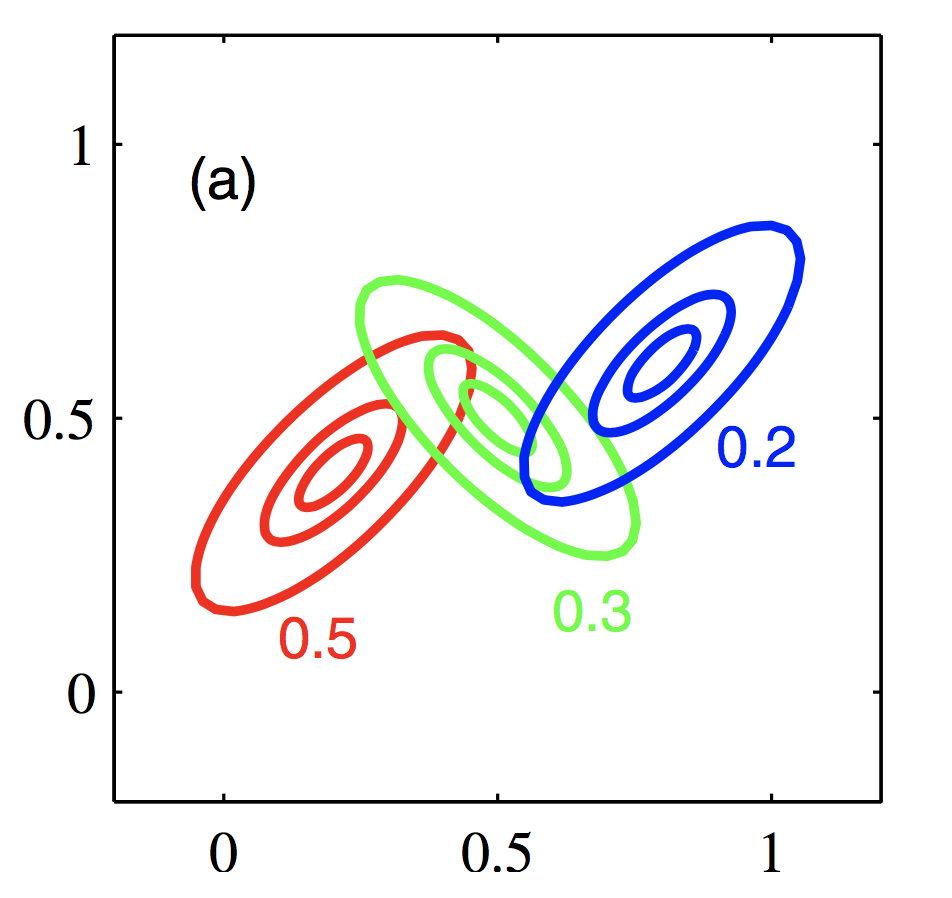
\includegraphics[width=0.75\linewidth]{figs/mixture_of_gaussians.png}
		\end{figure}
		\vspace{-0.5cm}
	    \begin{itemize}
	        \item $p(\bx | \bz, \btheta) = \mathcal{N}(\bx | \boldsymbol{\mu}_\bz, \boldsymbol{\Sigma}_\bz)$
	        \item $p(\bz) = \text{Categorical}(\bz | \boldsymbol{\pi})$
	    \end{itemize}
	\end{minipage}%
	\begin{minipage}[t]{0.53\columnwidth}
		\textit{PCA model} \\
		\vspace{-0.5cm}
		\begin{figure}
			\centering
			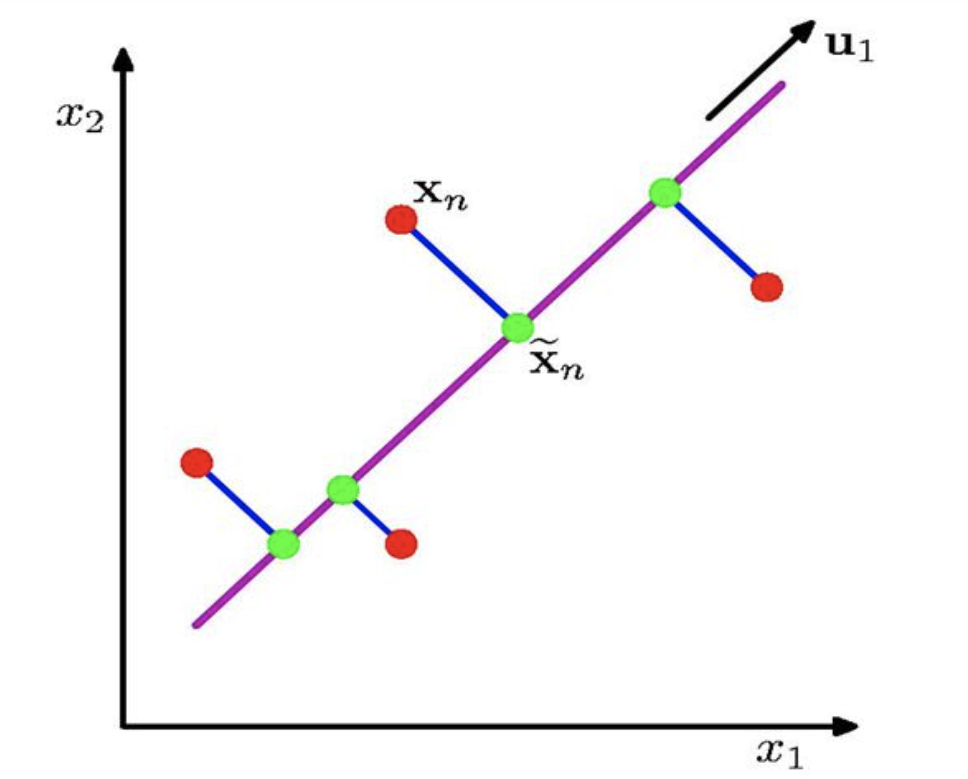
\includegraphics[width=.7\linewidth]{figs/pca.png}
		\end{figure}
		\vspace{-0.5cm}
		\begin{itemize}
	        \item $p(\bx | \bz, \btheta) = \mathcal{N}(\bx | \mathbf{W} \bz + \boldsymbol{\mu}, \boldsymbol{\Sigma}_\bz)$
	        \item $p(\bz) = \mathcal{N}(\bz | 0, \mathbf{I})$
	    \end{itemize}
	\end{minipage}
	\end{block}
\myfootnote{Bishop\,C. Pattern Recognition and Machine Learning, 2006}
\end{frame}
%=======
\begin{frame}{Latent variable models (LVM)}
    \[
    \log p(\bx | \btheta) = \log \int p(\bx | \bz, \btheta) p(\bz) d\bz \rightarrow \max_{\btheta}
    \]
	\textbf{PCA goal:} Project original data $\bX$ onto a low dimensional latent space while maximizing the variance of the projected data. 
	\begin{figure}
		\centering
		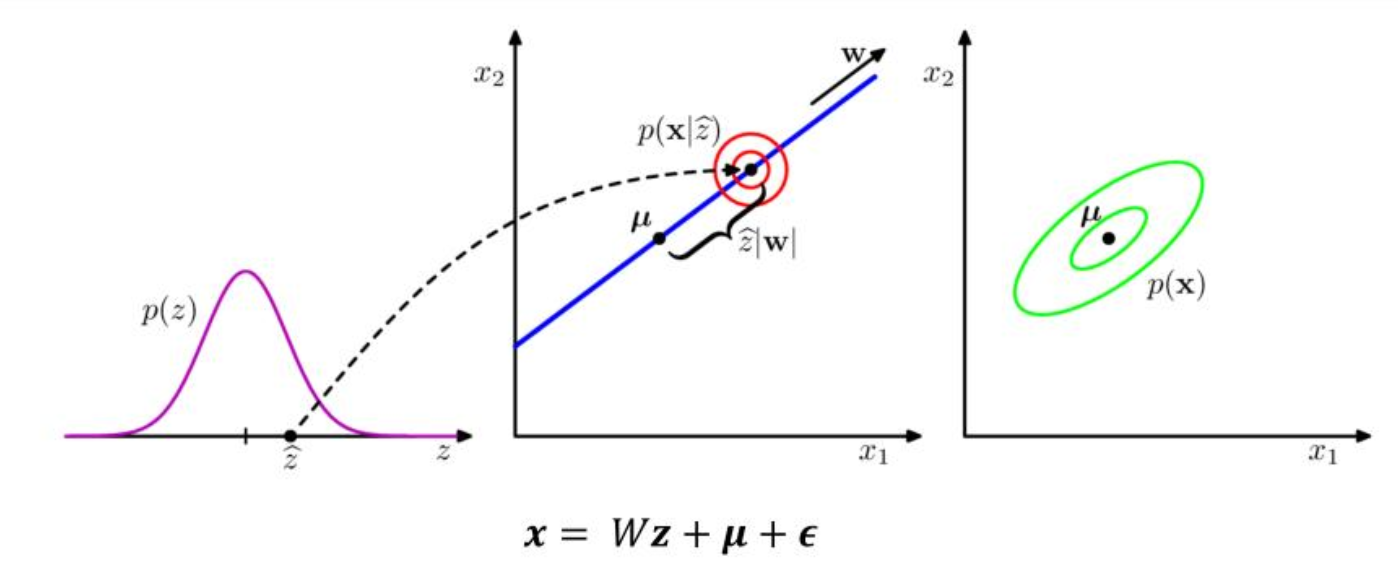
\includegraphics[width=.7\linewidth]{figs/bayesian_pca.png}
	\end{figure}
	\vspace{-0.5cm}
	\begin{itemize}
        \item $p(\bx | \bz, \btheta) = \mathcal{N}(\bx | \mathbf{W} \bz + \boldsymbol{\mu}, \boldsymbol{\Sigma}_\bz)$
        \item $p(\bz) = \mathcal{N}(\bz | 0, \mathbf{I})$
    \end{itemize}
    
    \myfootnote{Bishop\,C. Pattern Recognition and Machine Learning, 2006}
    
\end{frame}
%=======
\begin{frame}{Incomplete likelihood}
        \begin{block}{MLE}
            \vspace{-0.7cm}
            \begin{multline*}
                \vspace{-0.5cm}
                \btheta^* = \argmax_{\btheta} p(\bX, \bZ | \btheta) = \argmax_{\btheta} \prod_{i=1}^n p(\bx_i, \bz_i | \btheta) = \\ = \argmax_{\btheta} \sum_{i=1}^n \log p(\bx_i, \bz_i | \btheta).
            \end{multline*}
            \vspace{-0.5cm}
        \end{block}
	Since $\bZ$ is unknown, maximize \textbf{incomplete likelihood}.
    \begin{block}{MILE problem}
        \vspace{-0.7cm}
    	\begin{multline*}
        	\btheta^* = \argmax_{\btheta} \log p(\bX| \btheta) = \argmax_{\btheta} \sum_{i=1}^n \log p(\bx_i | \btheta) = \\ =  \argmax_{\btheta}  \sum_{i=1}^n \log \int p(\bx_i, \bz_i | \btheta) d \bz_i = \\ = \argmax_{\btheta} \log \int p(\bx_i| \bz_i, \btheta) p(\bz_i) d\bz_i.
    	\end{multline*}
	\end{block}
	
\end{frame}
%=======
\begin{frame}{Variational lower bound}
	\begin{multline*}
		\log p(\bx| \btheta) 
		= \log \frac{p(\bx, \bz| \btheta)}{p(\bz|\bx, \btheta)} = \\ 
		= \int q(\bz) \log \frac{p(\bx, \bz| \btheta)}{p(\bz|\bx, \btheta)}d\bz
		= \int q(\bz) \log \frac{p(\bx, \bz| \btheta) q(\bz)}{p(\bz|\bx, \btheta) q(\bz)} d\bz = \\
		= \int q(\bz) \log \frac{p(\bx, \bz | \btheta)}{q(\bz)}d\bz + \int q(\bz) \log \frac{q(\bz)}{p(\bz|\bx, \btheta)}d\bz = \\ 
		= \mathcal{L} (q, \btheta) + KL(q(\bz) || p(\bz|\bx, \btheta)) \geq \mathcal{L} (q, \btheta).
	\end{multline*}
	\vspace{-0.5cm}
	\begin{block}{Kullback-Leibler divergence}
	    \begin{itemize}
	    	\item $KL(q || p) = \int q(\bz) \log \frac{q(\bz)}{p(\bz)} d \bz$;
	        \item $KL(q || p) \geq 0$;
	        \item $KL(q || p) = 0 \Leftrightarrow q \equiv p$.
	    \end{itemize}
	\end{block}
\end{frame}
%=======
\begin{frame}{Variational lower bound}
\[
    \log p(\bx| \btheta) = \mathcal{L} (q, \btheta) + KL(q(\bz) || p(\bz|\bx, \btheta)) \geq \mathcal{L} (q, \btheta).
\]
\begin{block}{Evidence Lower Bound (ELBO)}
\begin{align*}
    \mathcal{L} (q, \btheta) &= \int q(\bz) \log \frac{p(\bx, \bz | \btheta)}{q(\bz)}d\bz = \\ 
    &= \int q(\bz) \log p(\bx | \bz, \btheta) d\bz + \int q(\bz) \log \frac{p(\bz)}{q(\bz)}d\bz \\ 
    &= \mathbb{E}_{q} \log p(\bx | \bz, \btheta) - KL (q(\bz) || p(\bz))
\end{align*}
\end{block}
Instead of maximizing incomplete likelihood, maximize ELBO (equivalently minimize KL)
\[
    \max_{\theta} p(\bx | \btheta) \quad \rightarrow \quad \max_{q, \theta} \mathcal{L} (q, \btheta) \equiv \min_{q, \theta} KL(q(\bz) || p(\bz|\bx, \btheta)).
\]
    
\end{frame}
%=======
\begin{frame}{EM-algorithm}
	\[
		\mathcal{L} (q, \btheta)  = \int q(\bz) \log p(\bx | \bz, \btheta) d\bz + \int q(\bz) \log \frac{p(\bz)}{q(\bz)}d\bz.
	\]
	\begin{block}{Block-coordinate optimization}
	\begin{itemize}
		\item Initialize $\btheta^*$;
		\item E-step
		\[
			q(\bz) = \argmax_q \mathcal{L} (q, \btheta^*) = \argmin_q KL(q || p) =
			 p(\bz| \bx, \btheta^*);
		\]
		\item M-step
		\[
			\btheta^* = \argmax_{\btheta} \mathcal{L} (q, \btheta);
		\]
		\item Repeat E-step and M-step until convergence.
	\end{itemize}
	\end{block}
\end{frame}
%=======
\begin{frame}{Ugly pic}
\end{frame}
%=======
\begin{frame}{Amortized variational inference}
    \begin{block}{E-step}
    \vspace{-0.3cm}
    \[
		q(\bz) = \argmax_q \mathcal{L} (q, \btheta^*) = \argmin_q KL(q || p) =
		 p(\bz| \bx, \btheta^*).
	\]
	\begin{itemize}
		\item $p(\bz| \bx, \btheta^*)$ could be \textbf{intractable};
		\item $q(\bz)$ is different for each object $\bx$.
	\end{itemize}
    \end{block}
	\begin{block}{Idea}
	Restrict a family of all possible distributions $q(\bz)$ to a particular parametric class $q(\bz|\bx, \bphi)$ conditioned on samples $\bx$ with parameters $\bphi$.
	\end{block}
	
	\textbf{Variational Bayes}
	\begin{itemize}
		\item E-step
		\[
		\bphi_k = \bphi_{k-1} + \left.\eta \nabla_{\bphi} \mathcal{L}(\bphi, \btheta_{k-1})\right|_{\bphi=\bphi_{k-1}}
		\]
		\item M-step
		\[
		\btheta_k = \btheta_{k-1} + \left.\eta \nabla_{\btheta} \mathcal{L}(\bphi_k, \btheta)\right|_{\btheta=\btheta_{k-1}}
		\]
	\end{itemize}
\end{frame}%=======
\begin{frame}{Variational EM-algorithm}

	\begin{block}{ELBO}
		\vspace{-0.1cm}
		\[
		\log p(\bx| \btheta) = \mathcal{L} (q, \btheta) + KL(q(\bz) || p(\bz|\bx, \btheta)) \geq \mathcal{L} (q, \btheta).
		\]
	\end{block}
	\begin{itemize}
		\item E-step
		\[
		\bphi_k = \bphi_{k-1} + \left.\eta \nabla_{\bphi} \mathcal{L}(\bphi, \btheta_{k-1})\right|_{\bphi=\bphi_{k-1}},
		\]
		where $\bphi$~-- parameters of variational distribution $q(\bz | \bx, \bphi)$.
		\item M-step
		\[
		\btheta_k = \btheta_{k-1} + \left.\eta \nabla_{\btheta} \mathcal{L}(\bphi_k, \btheta)\right|_{\btheta=\btheta_{k-1}},
		\]
		where $\btheta$~-- parameters of the generation function $p(\bx | \bz, \btheta)$.
	\end{itemize}
	Now all we have to do is to obtain two gradients $\nabla_{\bphi} \mathcal{L}(\bphi, \btheta)$, $\nabla_{\btheta} \mathcal{L}(\bphi, \btheta)$.  \\
	\textbf{Difficulty:} number of samples $n$.
\end{frame}
%=======
\begin{frame}{ELBO gradient (M-step, $\nabla_{\btheta} \mathcal{L}(\bphi, \btheta)$)}
	\vspace{-0.3cm}
	\[
		\sum_{i=1}^n \mathcal{L}_i (\bphi, \btheta)  = \sum_{i=1}^n \mathbb{E}_{q} \log p(\bx_i | \bz_i, \btheta) - KL (q(\bz_i| \bx_i, \phi) || p(\bz_i)) \rightarrow \max_{\bphi, \btheta}.
	\]
	Optimization w.r.t. $\btheta$: \textbf{mini-batching} (1) + \textbf{Monte-Carlo} estimation (2)
	\begin{align*}
		\nabla_{\btheta} \sum_{i=1}^n \mathcal{L}_i (\bphi, \btheta)
		&= \sum_{i=1}^n \int q(\bz_i|\bx_i, \bphi) \nabla_{\btheta}\log p(\bx_i|\bz_i, \btheta)  d \bz_i \\
		&\mathrel{\stackrel{\rm (1)}\approx} n\int q(\bz_i|\bx_i, \bphi) \nabla_{\btheta}\log p(\bx_i|\bz_i, \btheta) d \bz_i , \quad i \sim U[1, n] \\
		&\mathrel{\stackrel{\rm (2)}\approx}  n \nabla_{\btheta}\log p(\bx_i|\bz^*_i, \btheta), \quad \bz^*_i \sim q(\bz_i|\bx_i, \bphi).
	\end{align*}
	\textbf{Monte-Carlo} estimation (2):
	\[
		\bbE_q f(\bz) = \int q(\bz) f(\bz) d\bz \approx f(\bz^*), \text{where } \bz^* \sim q(\bz).
	\]
	\end{frame}
%=======
\begin{frame}{ELBO gradient (E-step, $\nabla_{\bphi} \mathcal{L}(\bphi, \btheta)$)}
	\vspace{-0.3cm}
	\[
	\sum_{i=1}^n \mathcal{L}_i (\bphi, \btheta)  = \sum_{i=1}^n \mathbb{E}_{q} \log p(\bx_i | \bz_i, \btheta) - KL (q(\bz_i| \bx_i, \phi) || p(\bz_i)) \rightarrow \max_{\bphi, \btheta}.
	\]
	Difference from M-step: density function $q(\bz| \bx, \bphi)$ depends on the parameters $\bphi$, it is impossible to use the Monte-Carlo estimation:
	\[
	\nabla_{\bphi} \mathcal{L} (\bphi, \btheta) = \int \nabla_{\bphi} q(\bz| \bx, \bphi) \log p(\bx |\bz, \btheta) d\bz - \nabla_{\bphi} KL
	\]
	
	First term is not an expectation due to the gradient.
	
	\begin{block}{Possible solutions}
		\begin{itemize}
			\item log-derivative trick;
			\item reparametrization trick.
		\end{itemize}
	\end{block}
\end{frame}
%=======
\begin{frame}{ELBO gradient (E-step, $\nabla_{\bphi} \mathcal{L}(\bphi, \btheta)$)}
	\begin{block}{Log-derivative trick}
		\vspace{-0.3cm}
		\[
		\nabla_\xi q(\eta| \xi) = q(\eta | \xi) \left( \frac{\nabla_\xi q(\eta | \xi)}{q(\eta| \xi)} \right) = q(\eta | \xi) \nabla_\xi \log q(\eta| \xi).
		\]
		\[
		\nabla_{\bphi} q(\bz| \bx, \bphi) = q(\bz| \bx, \bphi) \nabla_{\bphi} \log q(\bz| \bx, \bphi).
		\]
	\end{block}
	\begin{block}{ELBO}
		\vspace{-0.5cm}
		\begin{multline*}
			\nabla_{\bphi} \sum_{i=1}^n \mathcal{L}_i (\bphi, \btheta) = \sum_{i=1}^n \int \nabla_{\bphi} q(\bz_i| \bx_i, \bphi) \log p(\bx_i |\bz_i, \btheta) d\bz_i  - \nabla_{\bphi} KL \\ 
			= \sum_{i=1}^n \int q(\bz_i | \bx_i, \bphi) \bigl[  \nabla_{\bphi} \log q(\bz_i| \bx_i, \bphi) \log p(\bx_i |\bz_i, \btheta) \bigr] d\bz_i - \nabla_{\bphi} KL \\ \approx n \nabla_{\bphi} \log q(\bz_i^*| \bx_i, \bphi) \log p(\bx_i |\bz_i^*, \btheta) - \nabla_{\bphi} KL, \quad \bz_i^* \sim q(\bz_i| \bx_i, \bphi).
		\end{multline*}
	\end{block}
	\vspace{-0.2cm}
	\begin{block}{Problem} 
		Unstable solution with huge variance.
	\end{block}
\end{frame}
%=======
\begin{frame}{ELBO gradient (E-step, $\nabla_{\bphi} \mathcal{L}(\bphi, \btheta)$)}
	\begin{block}{Reparametrization trick}
		\vspace{-0.3cm}
		\[
		f(\xi) = \int q(\eta|\xi) h(\eta) d\eta
		\]
		Let $\eta = g(\xi, \epsilon)$, where $g$ is a deterministic function, $\epsilon$ is a random variable with a density function $r(\epsilon)$.
		\begin{multline*}
			\nabla_\xi \int q(\eta|\xi) h(\eta) d\eta = \nabla_\xi \int r(\epsilon) h(g(\xi, \epsilon)) d \epsilon \\
			\approx \nabla_\xi h(g(\xi, \epsilon^*)), \quad \epsilon^* \sim r(\epsilon).
		\end{multline*}
	\end{block}
	\vspace{-0.1cm}
	\begin{block}{Example}
		\vspace{-0.3cm}
		\[
		q(\eta|\xi) = \mathcal{N}(\eta| \mu, \sigma^2), \quad r(\epsilon) = \mathcal{N}(\epsilon|0, 1), \quad \eta = \sigma \cdot \epsilon + \mu, \quad \xi = [\mu, \sigma].
		\]
	\end{block}
\end{frame}
%=======
\begin{frame}{ELBO gradient (E-step, $\nabla_{\bphi} \mathcal{L}(\bphi, \btheta)$)}
	\vspace{-0.3cm}
	\begin{multline*}
		\nabla_{\bphi} \sum_{i=1}^n \mathcal{L}_i (\bphi, \btheta) =  \sum_{i=1}^n \nabla_{\bphi}\int q(\bz_i|\bx_i, \bphi) \log p(\bx_i| \bz_i, \btheta)d\bz_i  - \nabla_{\bphi} KL \\ \approx  n \nabla_{\bphi}\int r(\bepsilon) \log p(\bx_i| g(\bx_i, \bepsilon, \bphi), \btheta)d\bepsilon  - \nabla_{\bphi} KL,\quad i \sim U[1, n]   \\ \approx
		n \nabla_{\bphi} \log p(\bx_i| g(\bx_i, \bepsilon^*, \bphi), \btheta)  - \nabla_{\bphi} KL , \quad \bepsilon^* \sim r(\bepsilon).
	\end{multline*}
	
	\begin{block}{Variational assumption}
		\[
		q(\bz| \bx, \bphi) = \mathcal{N} (\bmu(\bx), \bsigma(\bx)).
		\]
		\[
		\bz = g(\bx, \bepsilon, \bphi) = \bsigma(\bx) \cdot \bepsilon + \bmu(\bx).
		\]
	\end{block}
	$\nabla_{\bphi} KL (q(\bz | \bx, \bphi) || p(\bz))$ has an analytical solution.
\end{frame}
%=======
\begin{frame}{Variational autoencoder (VAE)}
	\begin{block}{Final algorithm}
		\begin{itemize}
			\item pick $i \sim U[1, n]$;
			\item compute a stochastic gradient w.r.t. $\bphi$
			\begin{multline*}
				\nabla_{\bphi} \mathcal{L} (\bphi, \btheta) = n \nabla_{\bphi} \log p(\bx_i | g(\bx_i, \bepsilon^*, \bphi), \btheta) - \\ - \nabla_{\bphi} KL (q(\bz_i|\bx_i, \bphi) || p(\bz_i)), \quad \bepsilon^* \sim r(\bepsilon);
			\end{multline*}
			\item compute a stochastic gradient w.r.t. $\btheta$
			\[
			\nabla_{\btheta} \mathcal{L} (\bphi, \btheta) = n \nabla_{\btheta} \log p(\bx_i|\bz^*_i, \btheta), \quad \bz^*_i \sim q(\bz_i|\bx_i, \bphi);
			\]
			\item update $\btheta, \bphi$ according to the selected optimization method (SGD, Adam, RMSProp).
		\end{itemize}
	\end{block}
\end{frame}
%=======
\begin{frame}{Variational autoencoder (VAE)}
	\begin{itemize}
		\item Encoder $q(\bz | \bx, \bphi) = \text{NN}_e(\bx, \bphi)$ outputs $\bmu(\bx)$ and $\bsigma(\bx)$.
		\item Decoder $p(\bx | \bz, \btheta) = \text{NN}_d(\bz, \btheta)$ outputs parameters of the sample distribution.
	\end{itemize}
	\begin{figure}[h]
		\centering
		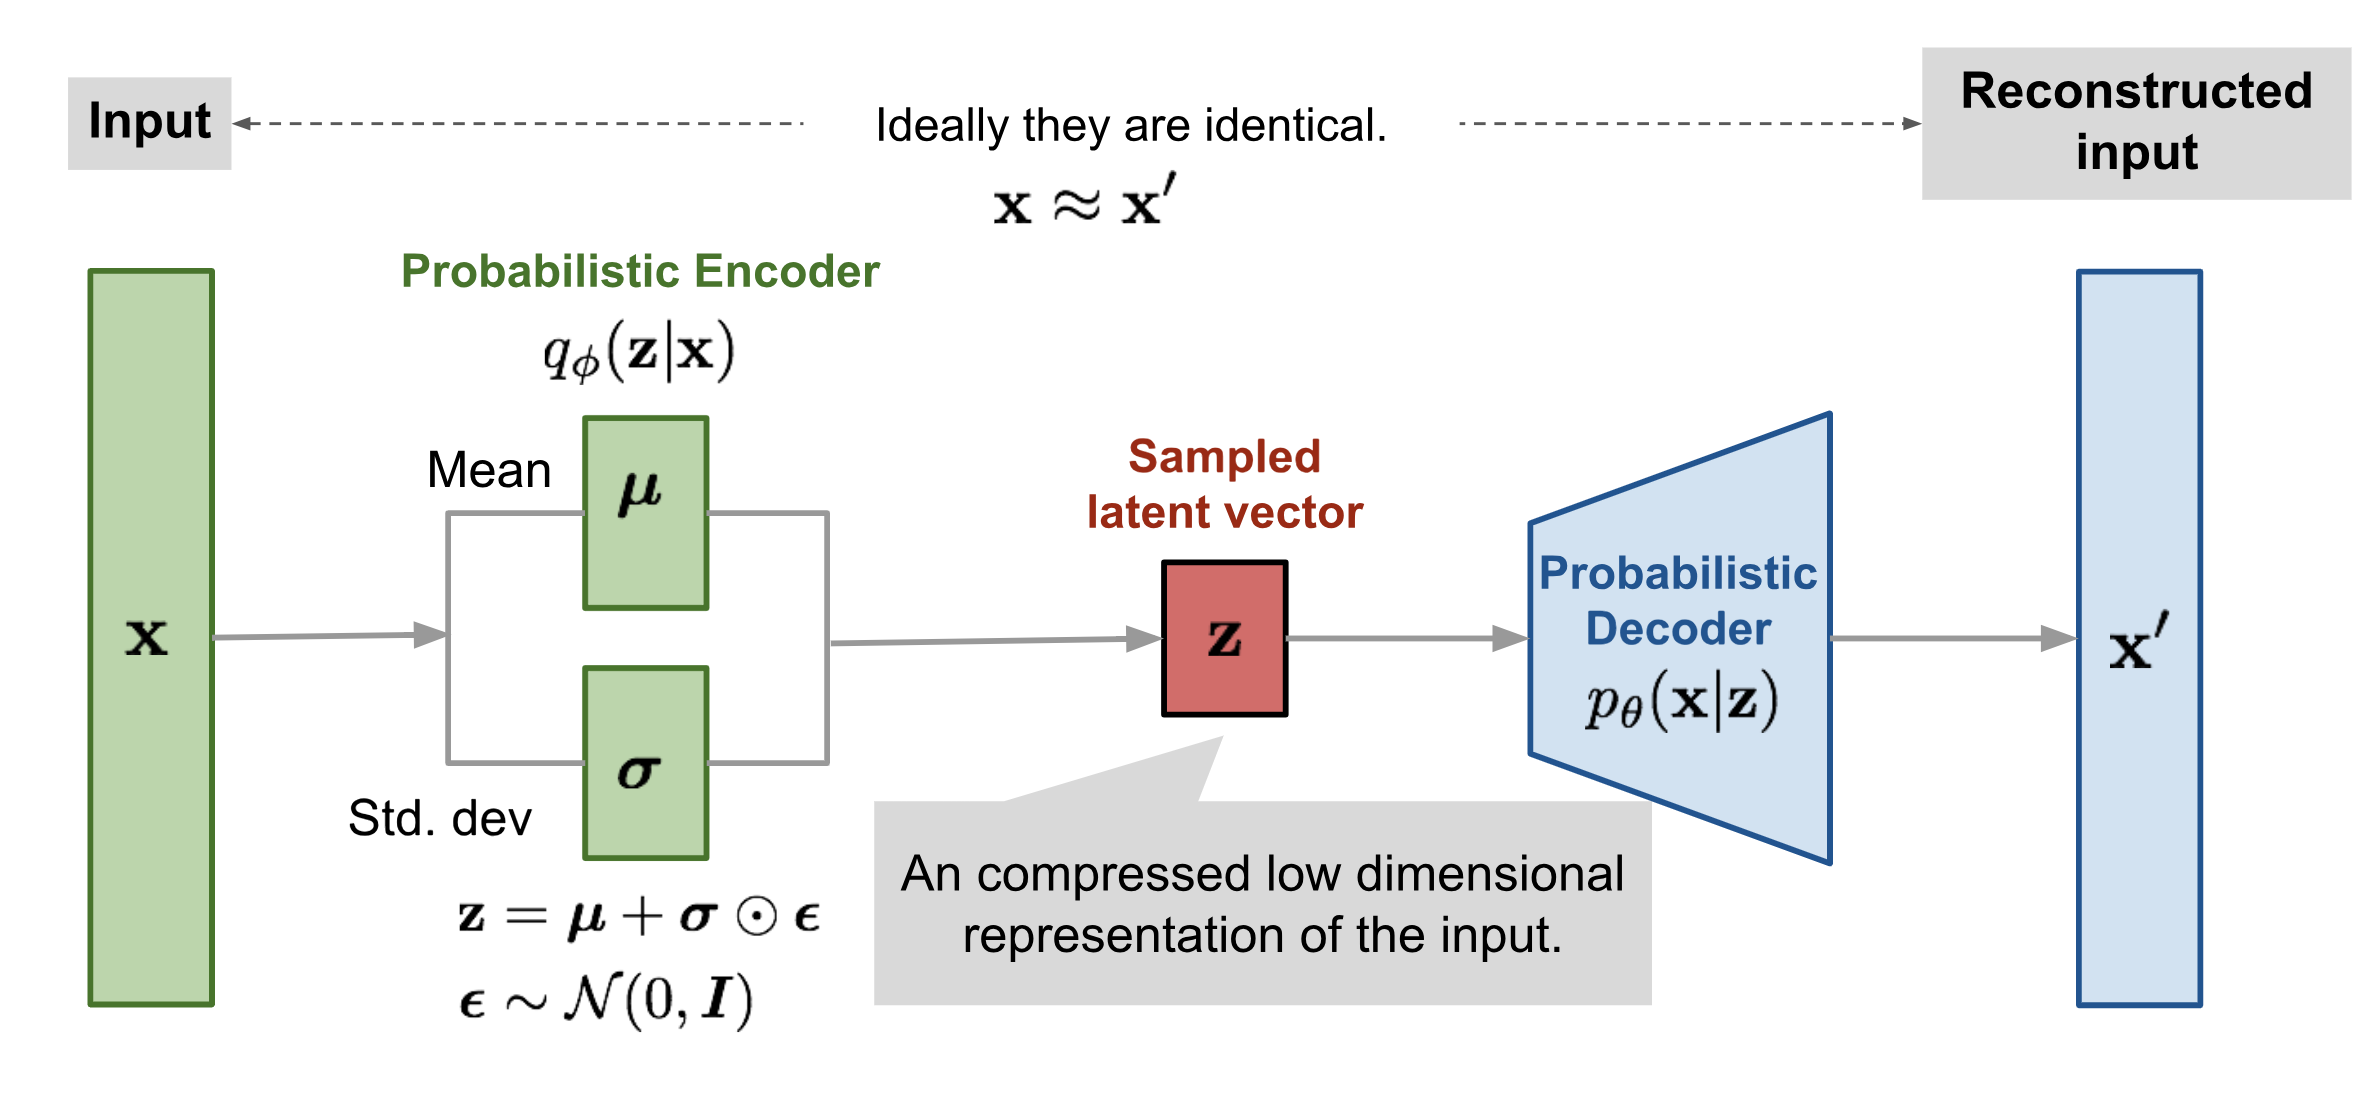
\includegraphics[width=\linewidth]{figs/vae-gaussian.png}
	\end{figure}
	
	\myfootnotewithlink{https://lilianweng.github.io/lil-log/2018/08/12/from-autoencoder-to-beta-vae.html}{image credit: https://lilianweng.github.io/lil-log/2018/08/12/from-autoencoder-to-beta-vae.html}
\end{frame}
%=======
\begin{frame}{Variational Autoencoder}
	\begin{figure}[h]
		\centering
		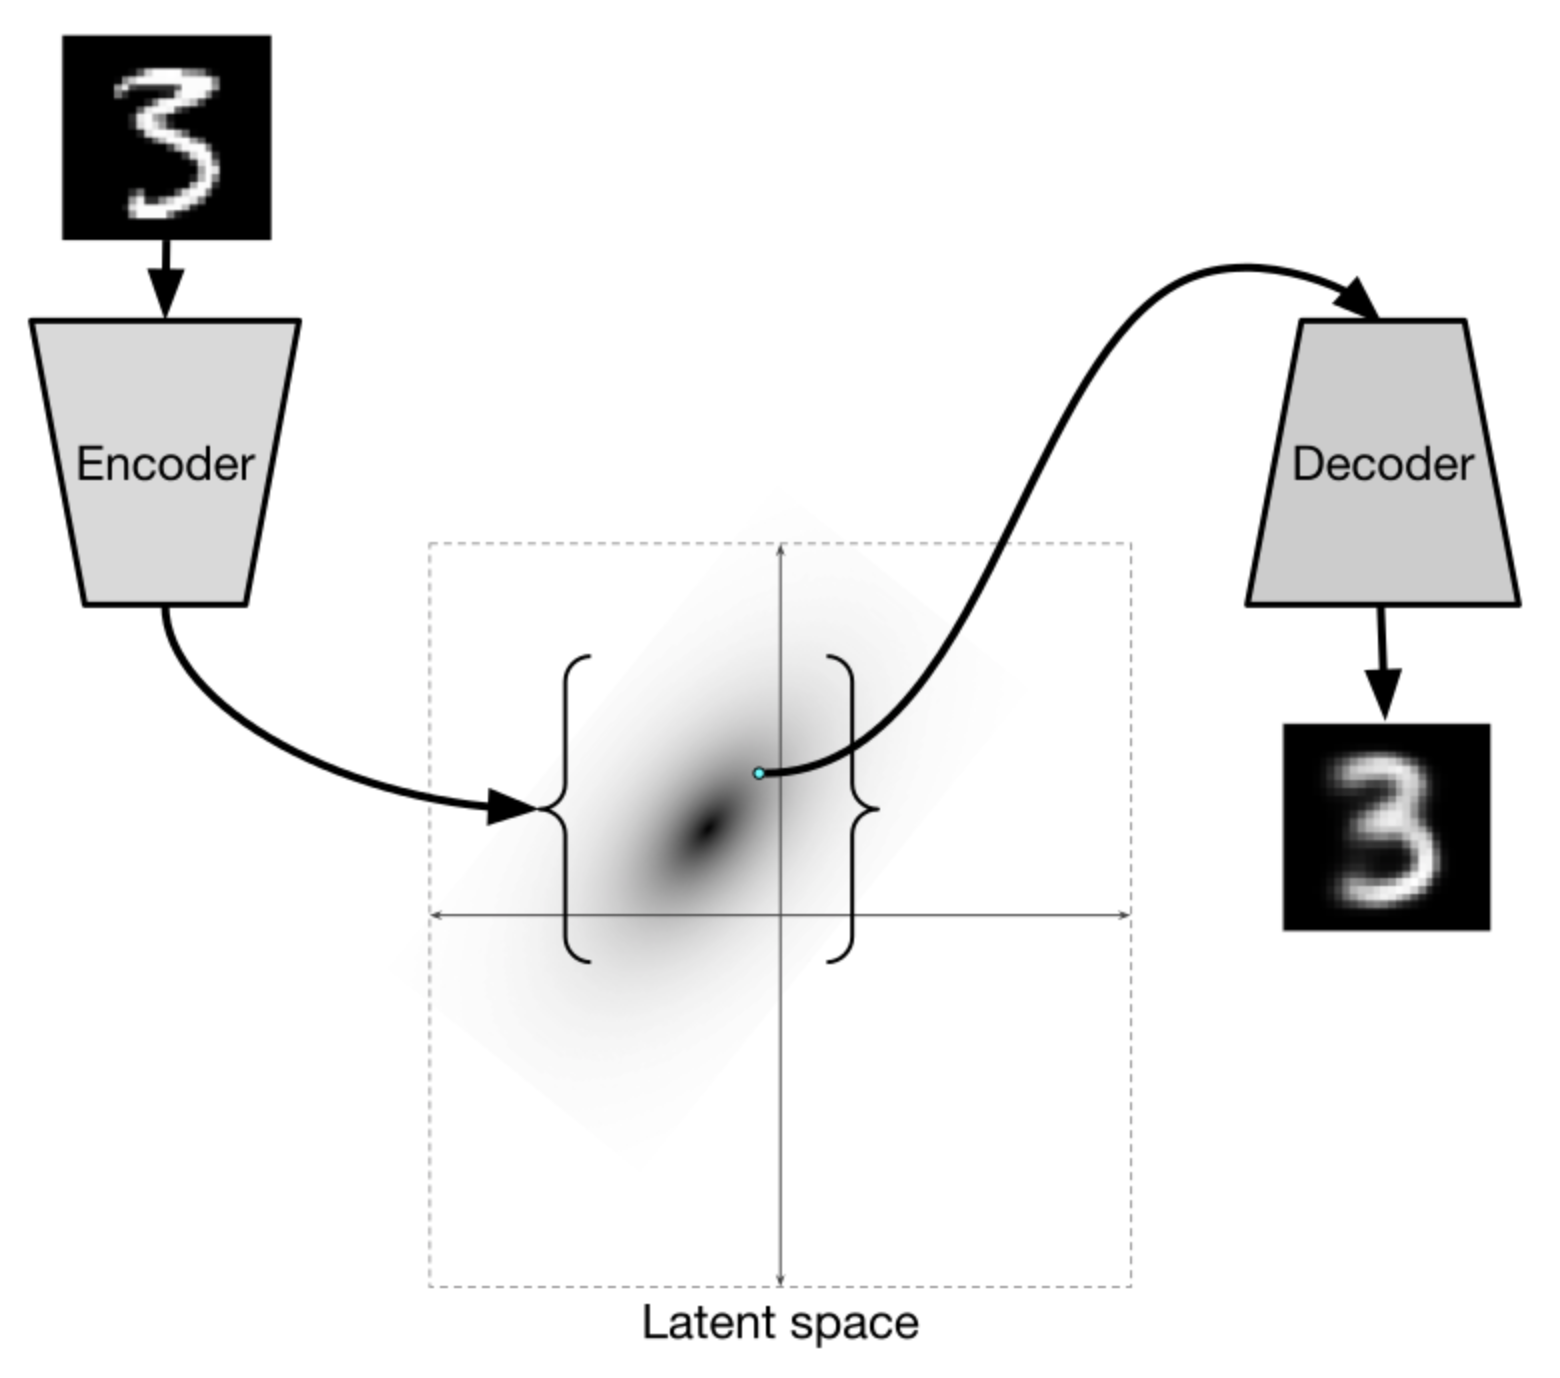
\includegraphics[width=.7\linewidth]{figs/VAE.png}
	\end{figure}
	\myfootnotewithlink{http://ijdykeman.github.io/ml/2016/12/21/cvae.html}{image credit: http://ijdykeman.github.io/ml/2016/12/21/cvae.html}
\end{frame}
%=======
\begin{frame}{Variational Autoencoder}
Generation objects by sampling the latent space $\bz \sim \mathcal{N}(0, \mathbf{I})$
\begin{figure}[h]
	\centering
	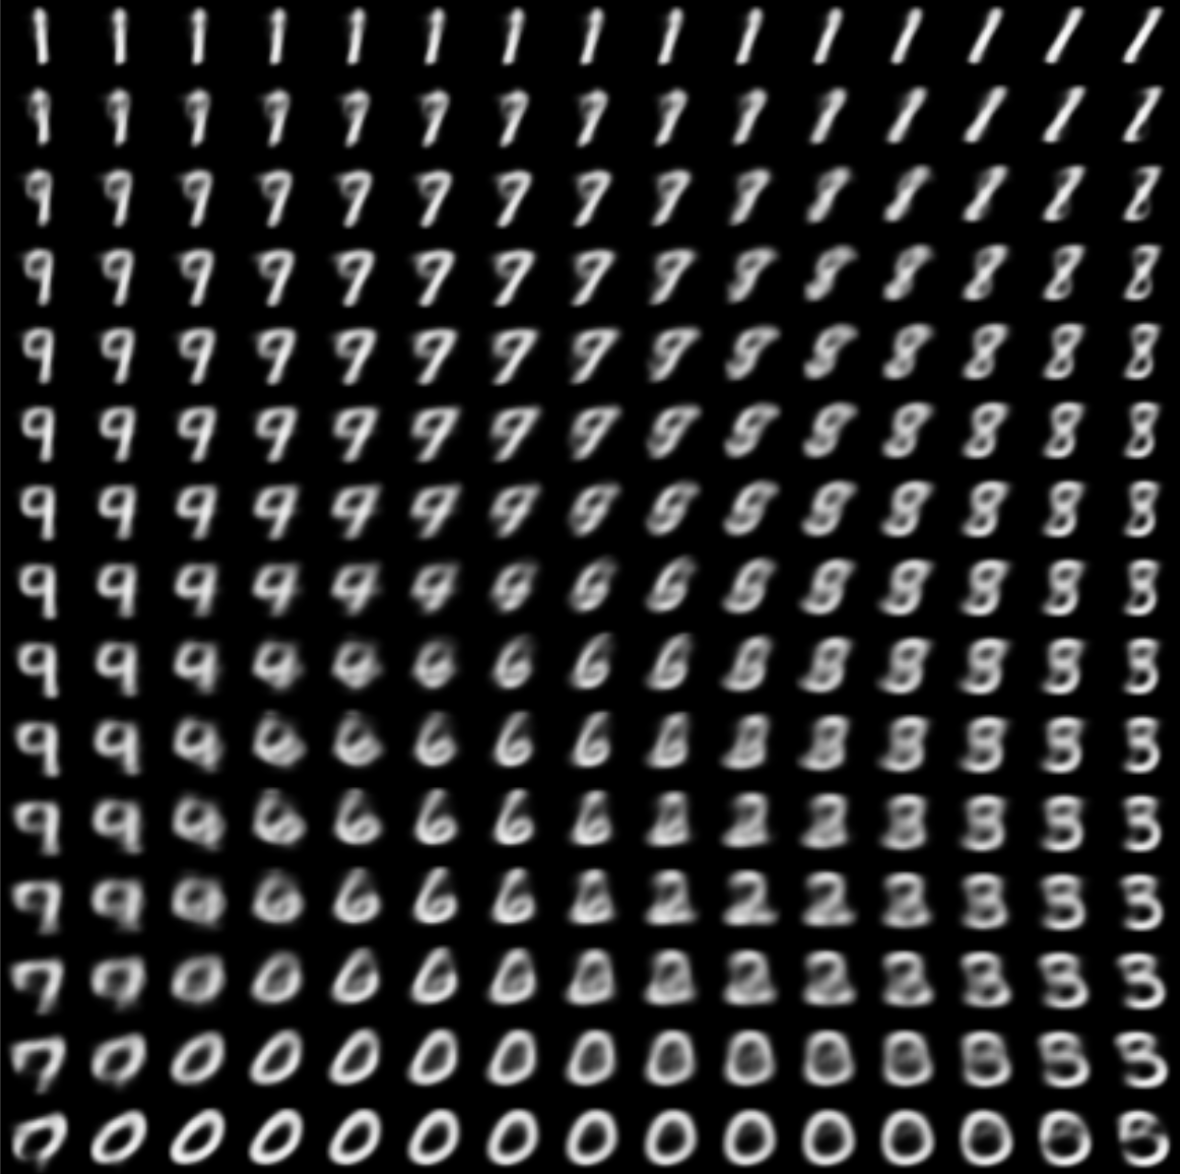
\includegraphics[width=.5\linewidth]{figs/vae_0.png}
\end{figure}
\myfootnotewithlink{https://habr.com/ru/post/331664}{image credit: https://habr.com/ru/post/331664}
\end{frame}
\begin{frame}{Summary}
	\begin{itemize}
		\item Bayesian inference is a generalization of most common machine learning tasks. It allows to construct MLE, MAP and bayesian inference, to compare models complexity and many-many more cool stuff.
		\item LVM introduce latent representation of observed samples to make model more interpretable.
		\item LVM maximizes variational evidence lower bound to find MLE of model parameters.
		\item ELBO maximization is performed by the general variational EM algorithm.
		\item Amortized inference allows to efficiently compute stochastic gradients for ELBO and to use deep neural networks for $q(\bz | \bx, \bphi)$ and $p(\bx | \bz, \btheta)$.
		\item The VAE model is an LVM with an encoder network for $q(\bz | \bx, \bphi)$ and a decoder network for $p(\bx | \bz, \btheta)$.
	\end{itemize}
\end{frame}
\end{document} 